%--------------------
%	CHAPTER 0
%--------------------

\chapterimage{chapter_head_1.pdf} % Chapter heading image

\chapter{Preliminaries}
If you see a mistake in this doc, or want further clarification somewhere, please make an in-line comment and I will fix, I made a macro for each of you to make colored comments: \\
\jjh{This is Jack's color}, \\
\dts{This is Dan's color},\\
\jsh{This is Jessie's color} \\ %% Use the command \jsh{ <insert comment here> } %% okie
\jap{This is Jake's color}\\
\kvdv{This is Kiki's color}
(see lines 57-61 newcommand definitions in the main.tex for this document)\\ \\
\noindent \jjh{(\href{https://www.dropbox.com/sh/759pwsjyc3ix0jy/AACv98R1Zpjvbaz2VhH4aH4ca?dl=0&fbclid=IwAR10ePsYI76S-MwDbBpH9fpoEbdxvyOlHs9PeaP2ZvY8SbJu1KPTxjMissA}{The Dropbox folder for this course can be found here, Homework sets, a copy of this text (updated regularly), and homework solutions will be posted as we go through the material.)}}\\

\jjh{\href{https://youtube.com/playlist?list=PLW3u28VuDAHJNrf3JCgT0GG_rjFVz0-j9}{Another wonderful resource as you venture further into this material are Dr. Aviv Censor's lectures on Algebra (Algebra 1M Technion University). Dr. Censor covers many topics featured in this book and uses very similar conventions to our book. Thank you Dr. Censor and Technion U for making these videos public!!!}}\\

\noindent Chapter 0 is meant to serve as a reference for symbols and terminology used in the main course material (Chapter 1 onward). On its own, this first Chapter is a doozy and we are gonna throw all sorts of new notation at you. Don't be intimidated. You do not need to understand or memorize all of this right away; the utility of these new notations will become apparent as you progress further through the text. Treat this chapter as a reference for the main course material that begins in Chapter 1. The authors recommend that readers who are familiar with mathematical induction already read sections 0.7 and 0.8. For readers who have never seen induction before, as to not distract from the more important intuition, we would prefer you skip 0.7 and 0.8 and read 0.8.1 first, then return to these sections after the underlying argument for the principle of induction is understood.

Lastly, when reading this material, read slowly and carefully and try to explain the argument out loud as if another were listening. Don't just read it aloud, really think about what the claim or statement is asserting. There is very little redundancy in mathematical writing so it pays dividends to read slowly, carefully, and to re-read many times until the argument is so clear that you could write it down again in your own words. When I read a new book or article in my field, the first 2-3 reads through I am just letting the new notations, jargon, definitions, and claims wash over me, I want to see the way the author uses these terms first and then I try to understand them more carefully. You can do it, you can piece it together! Just take baby steps to make your foundation solid.
\section{Common Notation seen in Herstein's book and this book}
$\blacksquare$ Denotes the end of a proof. Some authors  use the symbol \index{$\blacksquare$} $\square$\\ \\
$\exists$ read as `` There exists" \index{$\exists$} -- this symbol is commonly referred to as the ``existential quantifier"\\ \\
$\forall$ read as ``for all" \index{$\forall$} -- this symbol is commonly referred to as the ``universal quantifier"\\ \\
$\therefore \ $  read as ``therefore" \index{$\therefore$}\\ \\
$\because \ $ read as ``because" (we will use this symbol very rarely, usually we will just say "because")\\ \\
$a\in A$ read as ``$a$ is an element of $A$" or ``$a$ in $A$" \index{$\in$} \\ \\
$a\not\in A$ read as ``$a$ is \textit{not} an element of $A$" or ``$a$ not in $A$" \\ \\ \index{$\not\in$}
$\ni$ read as ``for which" or "who exhibits (\textit{pl.} exhibit ) the property..." or "who has (\textit{pl.} have ) the property..." \index{$\ni$}\\ \\

\begin{tcolorbox}
\begin{center}
NOTE: in this book \hl{$\in \neq \ni $}, i.e. "element of" and "element-wise for which" are \textit{not} the same symbol and  \underline{\hl{DO NOT mean the same thing}}.
\end{center}
\end{tcolorbox}
%or "who has (\textit{pl.} have ) the property" \\ \\ %(although some books will use $\in$ and $\ni$ interchangeably)
$| \ \ $ also read as ``for which" or "who exhibit the property..." or "who have the property..."; however this will almost always be used when referring to \textit{collections/sets} of elements "for which" a property holds (i.e. not element-wise), e.g. 
\begin{align}
    \{x\in \Z | 22\leq x < 27\}  \nonumber \\
    &= \{ \text{the subset of $\Z$ for which members are $\geq 22$ AND $<27$} \} \nonumber \\
    &= \{22,23,24,25,26\}\nonumber
\end{align}
  \\ \\%or "who has (\textit{pl.} have ) the property" \\ \\ %(although some books will use $\in$ and $\ni$ interchangeably)
$a\in A \ni P(a)$ read as `` $a$ is an element of $A$ for which Property $P(a)$ is true"\\ \\
$\implies$ read as ``implies"\\ \\
$A\implies B$ can be read as any of the following equivalent ways: ``A implies B", ``if A then B", ``A only if B" \footnote{This is important, if you need clarification look \href{https://criticalthinkeracademy.com/courses/propositional-logic/lectures/51574}{here (link)}}. We sometimes also say "$A$ is \textit{sufficient} for $B$" or "$B$ is \textit{necessary} for $A$"\\ \\ 
$\Leftrightarrow$ read as ``is equivalent to" or ``if and only if", also commonly written ``iff"\\ \\
If both ``$A$ only if $B$" is true (i.e. $A\implies B$, or, $A$ is true only if $B$ is true) and ``if $B$ then $A$" is true (i.e. $B\implies A$, or, if $B$ is true, then $A$ is true), then we say ``$A$ if and only if $B$" or "$A\iff B$" and the statements $A$ and $B$ are equivalent (see below). In this scenario we may also say "$A$ is \textit{necessary and sufficient} for $B$" or "$B$ is \textit{necessary and sufficient} for $A$" \\ \\
$A\iff B$ can also be read as ``$A$ if and only if $B$", ``$B$ if and only if $A$", ``$A$ iff $B$", ``$B$ iff $A$", ``$A$ is equivalent to $B$", ``$B$ is equivalent to $A$" lastly, this expression could also be read `` $A$ implies $B$ and $B$ implies $A$" or "$B$ implies $A$ and $A$ implies $B$". We emphasize the last two interpretations because iff statements (i.e. statements that use $\iff$) should be thought of as pairs of implications, one implication $LHS\implies RHS$ and another implication $RHS \implies LHS$. (LHS is left-hand-side here.)\\ \\
$\lnot A$ read ``not $A$" is called the negation of statement $A$ \\(e.g. $\lnot(\lnot A)\iff A$ and $x\neq y \iff \lnot(x=y)$ \ \ ) \\ \\
$\lnot B \implies \lnot A$ is called the contraposition of implication $A \implies B$. We have that $\lnot B \implies \lnot A \iff A\implies B$ (i.e. these expressions are equivalent, this is often useful for proofs, instead of proving $A\implies B$ we can prove $\lnot B \implies \lnot A$)\\ \\
The intuition for an implications equivalence with its contraposition is two parts: 
\begin{enumerate}
    \item ``If $B$ is \textit{always} true when $A$ is true ($A\implies B$), then if $B$ isn't true, $A$ must not be true ($\lnot B \implies \lnot A$)".
    \item ``If $A$ is \textit{always} false when $B$ is false ($\lnot B \implies \lnot A$), then if $A$ is true, $B$ must be true ($A\implies B$)".
\end{enumerate}
Examples of proof by contrapositive and proof by contradiction are given in the sub-sections below. \\ \\

\noindent In this text, the shorthand for ``contradiction" is a pair of arrows running into one another ``$\Rightarrow\Leftarrow$" so read this as ``contradiction".
\section{A Word About Axioms in This Book}
As of January 11th, 2021, Merriam-Webster defines the noun ``Axiom" as:
\begin{enumerate}
    \item ``a statement accepted as true as the basis for argument or inference"
    \item ``an established rule or principle or a self-evident truth".
    \item ``a maxim widely accepted on its intrinsic merit". Where, here, maxim means ``a general truth, fundamental principle, or rule of conduct".
\end{enumerate}
In the land of Mathematics, the meaning of the word ``Axiom" most closely resembles the definition given in 1. ; i.e. Axioms are statements which are assumed to be true and used as the basis for argument or inference \textit{without} justification. 

This book is not a set theory or foundations of mathematics course so we will take a \textit{few} things for granted. In this book, we will not attempt to define or construct the most fundamental tools that we begin our studies with: Sets and Integers (the set $\Z$ and properties of its elements). We will instead take these to be primitive notions that do not need justification. You can take a set to be a collection of objects, \textit{with no repeated objects}. You can also take the following facts about integers as axioms:
\noindent\begin{align}
    a,b\in \Z &\implies a+b\in \Z  \ \ \ &\text{i.e. it is always true that the sum of two integers is an integer}\nonumber \\
    \text{ and } &\implies a-b\in \Z \ \ \ &\text{i.e. it is always true that the difference of two integers is an integer}\nonumber \\
    \text{ and } &\implies \exists \ -a,-b \in \Z \ \ \ &\text{i.e. every integer has an additive opposite or "negative" that is an integer}\nonumber \\
     \text{ and } &\implies a\cdot b\in \Z \ \ \ &\text{i.e. the product of two integers is always an integer}\nonumber
\end{align} 
All of this being said, using the tools of first order logic that you will learn along the way, if you wished to, you could ``begin again" with some weaker assumptions and build your way back up to showing that e.g. adding, subtracting, or multiplying two integers gives another integer, or that every integer $a\in\Z$ has an opposite $-a\in\Z$. 

\section{Basic Set Theory Definitions}
Given a set $S$ we will consistently use the notation $A=\{a\in S\ |\ P(a)\}$ to read `` $A$ is the set of all elements in $S$ for which the property P is true". This notation is commonly referred to as \textbf{set builder} notation. We read the vertical bar `` $|$ " as ``for which" or sometimes ``such that", we will also commonly use the symbol $\ni$ to indicate ``for which" or ``such that" when we are referring to individual elements, e.g. $a\in A \ni a>0$ is read as `` $a$ is an element of $A$ for which $a>0$" or ``$a$ is an element of $A$ such that $a$ is greater than zero". \\ \\
\noindent Here is a simple example of this \textbf{set builder} notation in use, let $P(a)=$ "$a \text{ is even}$". \\
Then $\{a\in \Z | P(a)\} = \{...,-4,-2,0,2,4,6,...\} = \{ \text{the set of all even integers}\}$ \\ \\
Sometimes, a colon, ``$:$", will be used in place of the vertical bar, ``$|$", in set builder notation.\\ \\
\noindent We will now present five basic, but very important, definitions from Set Theory. 
\begin{definition}[Subset]\index{$\subset$}
Set $A$ is a \textit{subset} of set $B$, denoted $A\subset B$, if every element of $A$ is an element of $B$, that is, if
\begin{align}
    x\in A \implies x\in B
\end{align}
$A\subset B$ is typically read as "$A$ contained in $B$" or "$B$ contains $A$" or "$A$ is a subset of $B$"
\end{definition}
A simple visual example of $A\subset B$ can be seen in Figure \ref{fig:Subset_example}.
\begin{figure}[h!]
    \centering
    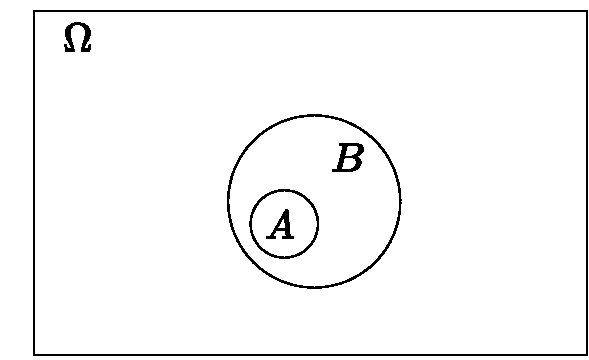
\includegraphics[width=0.5\textwidth]{Figures/SUBSET_Example.pdf}
    \caption{$A$ is a subset of $B$ since each element of $A$ is an element of $B$.}
    \label{fig:Subset_example}
\end{figure}\\
To define a set, we start with some “universe” of all possible elements of that set, usually called the \textit{universe of discourse} or simply \textit{universe}. In the figure above, our universe is denoted by $\Omega$. Then, a set $S$ can be defined by specifying which elements of the universe of discourse is in that set $S$, typically done with the set builder notation that we just introduced.
\begin{definition}[Set equality]
Sets $A$ and $B$ are equal if both $A\subset B$ and $B\subset A$
\end{definition}

\begin{definition}[Union of Sets] \index{$\cup$}
The \textit{union} of the two sets $A$ and $B$, written as $A\cup B$, is the set \\ $A\cup B = \{x\in \Omega |x\in A \text{ or } x\in B \}$ \steezybreak \\
\end{definition}
Let's read the above definition of $A\cup B$ in more regular speech, this equation says "A union B equals the set of elements $x$ for which $x$ is a member of A \textbf{or} $x$ is a member of B" we are using "$x$" here as a \textit{variable} and we mean that any such member $x$ who is either in $A$ \textbf{or} in $B$ (or possibly both!) is a member of this set $A$ union $B$. \\ \\
Figure \ref{fig:set_union_example} depicts a the union of two sets, $A$ and $B$.
\begin{figure}[h!]
    \centering
    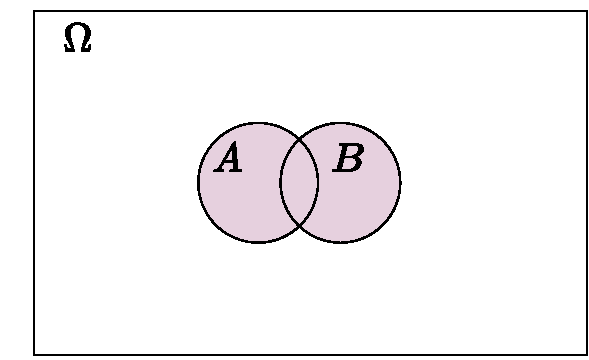
\includegraphics[width=0.5\textwidth]{Figures/Set_Union.pdf}
    \caption{The shaded region is $A\cup B$. $A\cup B$ is the set of all elements that are either in $A$ or in $B$.}
    \label{fig:set_union_example}
\end{figure}
\begin{definition}[Intersection of Sets]\index{$\cap$}
The \textit{intersection} of the two sets $A$ and $B$, written as $A\cap B$, is the set \\$A\cap B=\{x \in \Omega |x\in A \text{ and } x\in B \}$
\end{definition}
Let's read the above definition of $A\cap B$ in more regular speech, this equation says "$A$ intersect $B$ equals the set of elements $x$ for which $x$ is a member of $A$ \textbf{and} $x$ is a member of $B$". Again, we are using $x$ here as a variable and we mean that any element (who we choose to represent with the "handle" $x$) who satisfies $x$ in $A$ \textbf{and} $x$ in $B$ is a member of this set $A$ intersect $B$.\\ \\

\noindent Figure \ref{fig:set_intersection_example} depicts a the intersection of two sets $A$ and $B$.
\begin{figure}[h!]
    \centering
    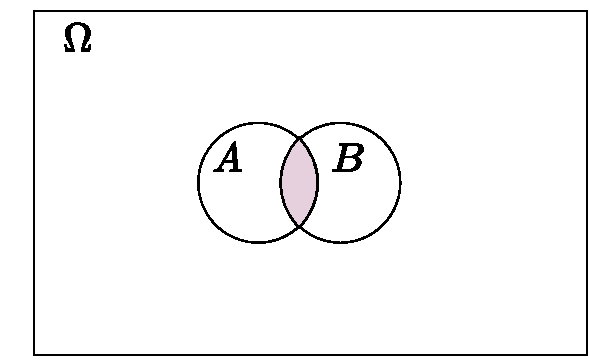
\includegraphics[width=0.5\textwidth]{Figures/Set_INTERSECTION.pdf}
    \caption{The shaded region is $A\cap B$. $A\cap B$ is the set of all elements that are both in $A$ \textit{and} in $B$.}
    \label{fig:set_intersection_example}
\end{figure}

\begin{definition}[Difference of Sets (Difference Set)]
Given two sets $A$ and $B$, then the \textit{difference set} written as $A - B$ or sometimes $A\setminus B$, is the set \\$A-B=\{x\in A| x\not\in B\}=\{x\in \Omega |x\in A \text{ and } x\not\in B \}$
\end{definition}
Note that we could define the difference set $A- B$ %lightly more generally by defining it in terms of some ``universe" set $\Omega$ who contains all the sets we are considering as subsets, i.e. $A,B \subset \Omega$. 
In another way using an idea known as set complement. In this case we would have $A- B=A\cap B^C$ where $B^C$ is referred to as the complement of set $B$ and it is defined as $B^C=\{x\in \Omega| x\not \in B\}$. For this reason, $A-B$ is sometimes called "the complement of $B$ in $A$". This form will almost never come up in this text but we mention it for interested readers who may go on to study Measure Theory (i.e. Probability), as it is an extremely convenient way to rewrite the difference of two sets when dealing with proofs in Measure Theory. 

\begin{figure}[h!]
    \centering
    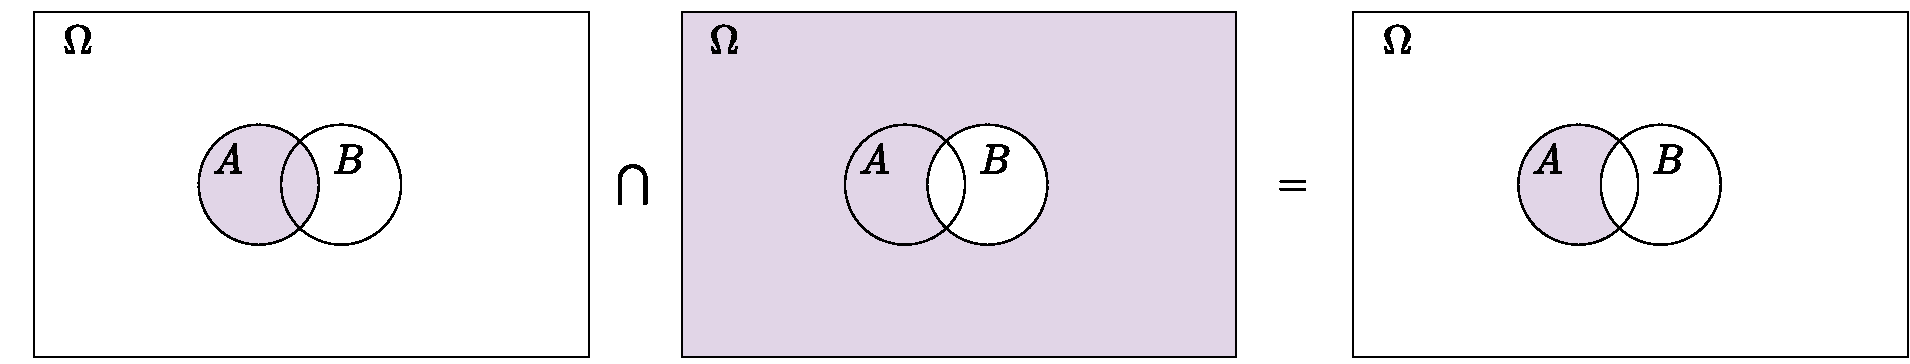
\includegraphics[width=0.9\textwidth]{Figures/Complements View of Set Minus.pdf}
    \caption{Complements View of Set Minus: on the left side of the intersection, set $A$ is shaded in, on the right side of the intersection set $B^C$ ($B$'s complement in universe $\Omega$) is shaded in, now it is easy to see that $A$'s intersection with $B^C$ (i.e. the portion these two shaded regions have in common) is simply $A-B$, or "the parts of $A$ that are not in $B$".}
    \label{fig:complements_view_set_minus}
\end{figure}
\newpage
\noindent For the two definitions provided below, the reader should note a finite union/intersection is the union/intersection of a finite number of sets; this phrase does not imply that the union/intersection set itself is a finite set!

\begin{definition}[Finite Union of Sets]
    A \textit{finite union} of sets $A_1, A_2, A_3, \dots , A_n$ could be written $A_1 \cup A_2 \cup A_3 \cup \dots \cup A_n$ (as union is associative) or, more commonly, $\bigcup_{i=1}^n A_i$. 
\begin{align}
    \bigcup_{i=1}^n A_i &= \{x\in \Omega \ | \ x\in A_1 \text{ or } x \in A_2 \text{ or } x\in A_3 \  \cdots \text{ or } x\in A_n\} \nonumber \\
    &= A_1 \cup A_2 \cup A_3 \cup \dots \cup A_n \nonumber 
\end{align}
%\textit{The second equality above can be proven using an induction argument and associativity of unions (which allows us to remove parentheses without ambiguity), some might enjoy proving this as an exercise, but it is not required. Same for the definition below and associativity of intersections}
\end{definition}

\begin{definition}[Finite Intersection of Sets]
    A \textit{finite intersection} of sets $A_1, A_2, A_3, \dots , A_n$ could be written $A_1 \cap A_2 \cap A_3 \cap \dots \cap A_n$ (as intersection is associative) or, more commonly, $\bigcap_{i=1}^n A_i$. 
\begin{align}
    \bigcap_{i=1}^n A_i &= \{x\in \Omega \ | \ x\in A_1 \text{ and } x \in A_2 \text{ and } x\in A_3 \ \cdots \text{ and } x\in A_n\} \nonumber \\
    &= A_1 \cap A_2 \cap A_3 \cap \dots \cap A_n \nonumber 
\end{align}
\end{definition}
\newpage
\noindent\section{Some important sets to remember}
% \begin{align}
% \emptyset=\{\} =\text{ The empty set (set with no elements, $\emptyset$ is trivially a subset of all sets) } \nonumber \\
% \text{Bool}= \{T,F\} \nonumber \\
% \mathbb{Z}=\{..,-3,-2,-1,0,1,2,3,...\}= \text{ the integers} \nonumber\\
% \mathbb{Q}=\{\frac{a}{b} \ | \  a,b \in \mathbb{Z} \ni b\neq 0\}= \text{ the rationals} \nonumber\\
% \mathbb{R}=\{\ ...c_1c_0.c_{-1}c_{-2}...\  | \ c_i\in \{0,1,2,3,4,5,6,7,8,9\} \ \forall  i  \}= \text{ the reals} \nonumber\\
% \text{sets } A, B \text{ are said to be disjoint if } A\cap B= \emptyset=\{\} \nonumber
% \end{align}

$\emptyset=\{\}$ The empty set (set with no elements, $\emptyset$ is trivially a subset of all sets since for any set, empty or non-empty, you can always consider the collection of \textit{none} of its elements, this is exactly the empty set) \index{$\emptyset$} \index{$\{\}$}\\
%$\text{Bool}= \{T,F\}$ \\
% Originally decided to let 0 be in N but since we've never really needed it I'm redefining now (10/26/2023) let me know if this change is in conflict with anything I wrote later lol
$\mathbb{N}=\{1,2,3,4,...\}$  = the natural numbers\\ 
$\mathbb{Z}=\{..,-3,-2,-1,0,1,2,3,...\}=$ the integers\\
$\mathbb{Q}=\{\frac{a}{b} \ | \  a,b \in \mathbb{Z} \ni b\neq 0\}$= the rationals \\
$\mathbb{R}=\{\ ...c_1c_0.c_{-1}c_{-2}...\  | \ c_i\in \{0,1,2,3,4,5,6,7,8,9\} \ \forall  i  \}=$ the reals\\ \\
\textit{Note:} We will use the following standard interval notation for \textit{interval subsets} of $\R$.\\ 
Let $a,b\in \R, a<b$ we denote the following sets:\\
$(a,b)= \{r\in \R | a<r<b \} \subset \R$,\\
$[a,b)= \{r\in \R | a\leq r<b \} \subset \R$, \\ 
$(a,b]= \{r\in \R | a< r\leq b \} \subset \R$, and lastly, \\
$[a,b]= \{r\in \R | a\leq r \leq b \} \subset \R$ \\ 

\noindent A key observation about the above interval notations is that square brackets, "$[$" or "$]$", are used when a given "endpoint" (i.e. $a$ or $b$) \textit{is} a member of the subset. Round brackets, "$($" or "$)$", are used when a given "endpoint" \textit{is not} a member of the subset. From examples above this means $a\not \in (a,b]$ but $b\in (a,b]$ and similarly $a,b\in [a,b]$, but $a\not \in (a,b)$ and $b \not \in (a,b)$.\\ \\
Sets $A, B$ are said to be disjoint if $A\cap B= \emptyset=\{\}$\\

\noindent Figure \ref{fig:disjoint_sets} depicts an example of two sets $A$ and $B$ that are \textit{disjoint}, that is, they share no elements and their intersection is the empty set.
\begin{figure}[h!]
    \centering
    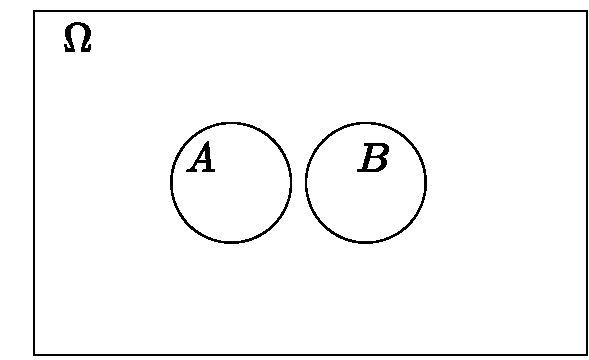
\includegraphics[width=0.5\textwidth]{Figures/disjoint_sets.pdf}
    \caption{$A$ and $B$ have no elements in common so $A\cap B=\emptyset$.}
    \label{fig:disjoint_sets}
\end{figure}

A collection of sets $A_1,A_2,...,A_n$ are said to be mutually disjoint if $A_i\cap A_j=\emptyset$ whenever $i\neq j$ \steezybreak \\


\section{Proof by Contrapositive Example} Let $x\in \mathbb{Z}$ and suppose we have statements $A=$``$x^2$ is even" and $B=$``$x$ is even", and wish to prove $A\implies B$, we can instead prove $\lnot B \implies \lnot A$ where $\lnot B=$``$x$ is not even" and $\lnot A=$``$x^2$ is not even". This latter statement is equivalent to the former and a proof by contraposition goes as follows: suppose that $x$ is not even, then $x$ is odd. The product of two odd numbers is odd, hence $x^2 = x\cdot x$ is odd. Thus $x^2$ is not even. Having proved the contrapositive, we can then infer that the original statement is true, i.e. that $A \implies B$ \\ \\
\href{https://www.math.toronto.edu/preparing-for-calculus/3_logic/we_3_negation.html}{Click Here for help with negating logical expressions. (See table at end of webpage)}\\

\noindent This is not to be confused with proof by contradiction. In proof by contradiction we have statement $A\implies B$ that we wish to show. To accomplish this, we begin by assuming $A$ is true \textit{and} that $B$ is false and we will arrive at a contradiction (notated as $\Rightarrow\Leftarrow$) that is a direct consequence of our incorrect assumption about $B$, meaning the only possibility is that our assumption about $B$ being false when $A$ is true was incorrect, meaning that if $A$ is true then $B$ must be true too, giving us the desired result: $A \implies B$ 
\noindent\section{Proof by Contradiction (a.k.a. 
\textit{Reductio ad absurdum}) Example:} In this example\footnote{ A reader who already knows some Category Theory and is fond of Type Theories may scoff at this example for Reductio ad absurdum as it relies on another (dubious?) tool (LOTEM). We will be working with Classical Logic for the time being, and under those rules, this is all fine. I may discuss introduction and elimination rules we've been using ( see Dr. Mark Jago's excellent lectures here: \textcolor{orange}{\href{https://www.youtube.com/watch?v=dlUkeN7KqVA&t=8s}{Propositional Logic/Classical Natural Deduction}/ \href{https://www.youtube.com/watch?v=C30w5vZypXE}{First-Order Logic}}) towards the end of the text and allude to logics that relax assumptions like double negation elimination. Stick with us, you may enjoy the presentation of the algebraic topics covered here \smiley } we will prove an implication using \textit{Reductio ad absurdum} or proof by contradiction. Given statements $A= "x^2 \text{ is even}"$, and $B= "x \text{ is even}"$, we could show $A\implies B$ through the following contradiction: Assume $A$ true and $\lnot B$ true, that is assume ``$x^2 \text{ is even}$" and ``$x \text{ is not even}$", now since $x$ is odd, and the product of two odds is odd, $x\cdot x$ is odd, but $x\cdot x=x^2$ and $x^2$ was assumed even! $\Rightarrow\Leftarrow$ (contradiction!). What we have shown is that $\lnot B$ cannot be true when $A$ is true. So our only option left is to conclude that if $A$ is true, then $B$ is true, i.e. $A\implies B$ %Given statements $A=$``The match is burning" and $B=$``There is oxygen in the room" we could show $A\implies B$ through the following contradiction: Assume $A$ true and $\lnot B$ true, that is assume ``The match is burning" and ``there is not oxygen in the room", immediately we arrive at a contradiction because as any person who has snuffed a candle knows ``burning " cannot occur without oxygen $\Rightarrow \Leftarrow$ (arrows running into each other is used to indicated a contradiction) therefore $\lnot B$ cannot be true when $A$ is true. So we have pigeon-holed our option for the true-ness or false-ness of statement B which statement A is assumed to be true, so our only option left is to conclude that when $A$ is true, $B$ must be true, i.e. $A\implies B$\\ \\

\section{Proof by Induction Example} Mathematical induction is a technique of proof that is essentially used to prove that a statement $P(n)$ holds for \textit{every} natural number $n = 1, 2, 3, ...$ ; that is, the overall statement is a sequence of infinitely many cases $P(1), P(2), P(3), ...$ \\
\noindent A proof by induction consists of two cases. The first, the base case (or basis), proves the statement for $n = 1$ without assuming any knowledge of other cases. The second case, the induction step, proves that if the statement holds for any given case $n\geq 1$, then it must also hold for the next case $n + 1$. These two steps establish that the statement holds for every natural number $n$. The base case does not necessarily begin with $n = 1$, but often with $n = 0$, and possibly with any fixed natural number $n = N$, establishing the truth of the statement for all natural numbers $n \geq N$. Now we will give an example of this approach of proof in order to prove the following fact about sums of natural numbers:
\begin{align}
    \sum_{k=1}^{n} k = \frac{n(n+1)}{2} \ \ \ \forall n \in \N \nonumber
\end{align}
In the proof below we will begin by establishing the result for a \textit{base case} where $n=1$. Then, in the \textit{induction step}, we will \textit{assume} that it holds for some $n\geq 1$ and we will show that assuming this $\implies$ $n+1$ also satisfies the property. The base case, together with the induction step, show that the rule is obeyed by all natural numbers $n\geq 1$ in a domino sort of effect, since $n=1$ (base) case plus the induction step implies that $n=2$ holds, then $n=2$ plus induction step implies $n=3$ holds, and so on and so forth. The principle of induction is a formal statement of this intuitive reasoning.\\
\textit{Proof:}\\
\noindent\textit{Base case:} Let $n=1$, then it is obvious that $\sum_{k=1}^1 k = 1 = \frac{1\cdot(2)}{2}=1$\\
\textit{Induction step:} Suppose for $n\geq 1$ it is true that 
\begin{align}
    \sum_{k=1}^n k&=\frac{n(n+1)}{2}\nonumber\\ 
    \implies \sum_{k=1}^{n} k + (n+1)&=\frac{n(n+1)}{2} +(n+1)\nonumber\\ 
    &=\frac{n(n+1)}{2} +\frac{2}{2}(n+1)\nonumber\\
    &=\frac{n(n+1)+2(n+1)}{2} \nonumber \\
    &=\frac{(n+1)(n+2)}{2} \nonumber \\
    &=\frac{(n+1)((n+1)+1)}{2} \nonumber
\end{align}
Since $\sum_{k=1}^{n} k + (n+1)=\sum_{k=1}^{n+1} k$ we have shown that arbitrary $n\geq 1$ obeying the rule \textit{implies} that $n+1$ also obeys the rule. This induction step, along with the base case for $n=1$ completes the proof. $\blacksquare$
\smallbreak

\section{A common pitfall when first learning Proof by Induction}
%\noindent Having just covered the principle of mathematical induction, the authors want to emphasize that both of the steps used (i.e. the base case, and inductive step) play an \textit{equal role} in proof of the fact. We emphasize the importance of the \textit{base case} first and then will use an example to show how base case oversights can often reveal themselves in the inductive step. In particular, we emphasize that when choosing the base case, the proof-writer should ensure that the base case is satisfied because of a property that follows from the assumptions about the claim, and not from a property of the \textit{specific} base case that was chosen. \\

%\noindent When choosing the base case above you might notice that we chose $n=1$ instead of $n=0$, partly this is because the claim only pertained to $n>0$, but the other reason for this is because while, $n=0$ satisfies the rule, (i.e. $0(0+1)/2=0$, it satisfies the rule in a trivial way, because the $0$ on the left annihilates the $1/2$ on the right and the sum of $0$ numbers $k$ is itself 0. \\ \\
%\noindent To make this more clear, what if you wanted to prove the obviously false statement that for $n>0, n^3\leq n^2$. \\ \\
%\textit{Bad Base case:}\\
%If we chose $n=1$ to be our base case, we can see that we (\textit{trivially}) satisfy the claim since $1^3=1\leq 1^2 = 1$, if we continued in this way and go on attempting to show the induction step, we may even be able to obtain an (erroneous) proof of this (false) statement. This proof has begun erroneously because the base case was chosen without care. It satisfied the statement about natural numbers, not because it was a natural number who is greater than 0, but because it was the \textit{specific} natural number $1$ (who has the property that all of his powers are the same, $1$).\\

\noindent Let's have a look at another induction proof and  see how a sneaky oversight is made in the proof of the inductive step. The reader should note that \textit{up until} this oversight is made, the proof is valid. That is, this oversight, is the \textit{sole} reason this proof is false. \\ \\
\noindent \textit{False theorem:} All horses are the same color.\\ \\
\textit{An Erroneous Proof by induction:}\\ \\
$P(n)$ is the statement: In every set of horses of size $n>0$, all $n$ horses are the same color.\\ \\
\textit{Base Case or $P(1)$}: One horse is the same color as itself. This is true by inspection. \\
\textit{Induction Step}: Assume $P(n)$ for some $n\geq 1$. Since $\{H_1,...,H_n\}$ is a set of $n$ horses, the induction hypothesis applies to this set. Thus, all the horses in this set are the same color.
Since $\{ H_2,...,H_{n+1}\}$ is also a set of $n$ horses, the induction step likewise holds for this set. Thus, all the horses in this set are the same color too. Lastly we note that these sets have horse $H_2$ in common, therefore, all $n+1$ horses in $\{H_1,...,H_n,H_{n+1}\}$ are the same color. $\blacksquare$

%This proof can be thought of as being erroneous for 2 reasons and in some ways these reasons are tied to each other as the reader will see. 
%The first reason this proof is erroneous is because the base case was again chosen without care. It satisfied the statement about collections of horses trivially, because there was only one horse, i.e. in the same way that all things are the same color as themselves, not because it was a collection of $n>0$ horses. In fact, because of the specific base case that we chose, we sneakily manage to \textit{avoid considering} the overlap of two distinct horses $H_1$ and $H_2$ because such a case does not exist for a collection containing only one horse, we only need to confirm that our one horse is the same color as the other horses but there are no "other horses". If we had instead chosen a base case of $n=2$ we would have immediately seen that this statement is not true in general since $\{\text{A Black Stallion}, \text{A White Stallion}\}$ is a collection of $2$ horses that does not satisfy the statement. \\ \\
%The explanation in the above paragraph is a very typical explanation for how choosing a poor representative for the base case can lead to a nonsensical proof. 
So it appears all horses are the same color? Well, there is a mistake in this proof. Can you see what assumption was made without justification?\\ \\
In the last sentence of the \textit{induction step}, we said ``lastly, we note these sets have horse $H_2$ in common." This statement is not necessarily true, is it? Because $H_2 \in \{H_1,...,H_n\}$ is true if and only if $n\geq 2$! The only way we could be sure $H_2 \in \{H_1,...,H_n\}$ is if $n\geq 2$ but we only assumed our $n\geq 1$, meaning $n$ could equal $1$ and then all bets are off about $H_2$ belonging to set $\{H_1,...,H_n\}$. If we take another tack, by instead trying to let our base case be $n=2$ and then make the induction for $n\geq 2$, we would immediately run into a problem. The problem we would encounter is that there are plenty of counter-examples which show the property does not hold for $n=2$ (e.g. $\{\text{A White Stallion},\text{A Black Stallion}\}$ is a collection of $2$ horses that does not satisfy the statement.) so we would be unable to prove our base case. Since we can find even \textit{one} counter-example, it must not be true for \textit{all} sets of horses of size $n$. \\

\noindent Whenever you are asked to prove or disprove a conjecture or claim, if you don't have a feeling about whether the conjecture is right or wrong (true or false) then you should start with some examples.  Either you will find a counter-example (disproving the claim) or you'll start to convince yourself that it's true.  Once you start to believe a conjecture and see a pattern then you can start to try to formulate a proof.  If you find that your proof isn't really coming together, then you can start to ask where it fails which, again, might lead you to a counter-example.
% The heart of our misunderstanding has now been laid bare and we can see that even having somewhat carelessly chosen the base case, it \textit{was} still true that the sets $\{H_1\}$ and $\{H_2\}$ are both collections of $n\geq 1$ horses and in each of those "collection" the horses are all the same color. Our mistake was assuming that the first of these sets should have any more than just $H_1$ which we cannot be sure of (since $n$ could be $1$) since we assumed $n\geq 1$ after making our base step.\\
%The moral of the story is that we must take care when choosing both the base case and making the induction step and we must not assume things before we have shown them!\\ \\

%(If you want even more explaining read my comment in the Ch0\_IntroTopics.tex below this sentence)\\ \\

\subsection{Induction in Fewer Words (Taken from Chong/\.Zak An Intro to Optimization 4 ed.)}
The principle of mathematical induction may be stated as follows. \\ \\
Assume that a given property of positive integers, $P(\cdot)$, satisfies the following conditions:
\begin{itemize}
    \item The number 1 possesses this property.
    \item If the number $n$ possesses this property, then the number $n + 1$ possesses it too.
\end{itemize}
The principle of induction states that under these assumptions any positive integer possesses the
property.\\

The principle of induction is easily understood using the following intuitive argument. If the number
$1$ possesses the given property, then the second condition implies that the number $2$ possesses the
property. But, then again, the second condition implies that the number $3$ possesses this property, and so on. The principle of induction is a formal statement of this intuitive reasoning.
\newpage
\section{Negating Logical Expressions}
This table provides a resource for negating the most common types of expressions that we will encounter in this class:
\begin{center}
  \begin{tabular}{|c|c|}\hline
     \textbf{Statement: $S$} & \textbf{Negation of Statement: $\lnot S$}   \\ \hline
     $A$ or $B$ & $\lnot A$ and $\lnot B$  \\ \hline 
     $A$ and $B$ & $\lnot A$ or $\lnot B$  \\ \hline
     if $A$ then $B$ & $A$ and $\lnot B$  \\ \hline
     $\forall \ x, \ P(x)$ & $\exists \ x \ni \lnot P(x)$  \\ \hline
     $\exists \ x \ni \ P(x)$ & $\forall \ x, \lnot P(x)$  \\ \hline
\end{tabular}  
\end{center}

%% EVEN MORE EXPLAINING %%
% There are many work-arounds to see that this Theorem is obviously false. Two of these approaches include: 

% 1) redefine a ``set" of ``horses" to always have $n\geq 2$ horses (i.e. a set with a single horse is not a set of horses, it is set containing a single horse) this is sort of a semantically nit-picking approach because it exposes that part of our problem was thinking that a set of "horses" could have only 1 horse to begin with. However this approach doesn't generalize very well because sometimes we \textit{do} want to let a "set" of "horses" include sets with only 1 horse.  This approach is kind of OVERKILL and forces us to rephrase the statement used to show the theorem entirely... (there is nothing wrong with this statement intrinsically... we just need to be careful about what implications we draw from from such a statement when we began by considering a collection with only 1 horse.)

% The other alternative is: 

% 2) \textit{Recognize} that while in the case with one horse, this property is satisfied, for \textit{all} other cases it is not. Then since we want to show for $n>0$ we can show $n=1$ directly as we did but we will NOT treat this as our base case for the induction (We just have to cover $n=1$ case if we are going to make our base case $n=2$ since we wanted to show it holds for $n>0$ ). Having recognized this issue, and having taken care of the earlier numbers below (i.e. $n=1$) the \textit{non-trivial} base case ($n=2$), we will instead set the base case to be $n=2$ and the false-ness of the claimed theorem is immediately apparent as this base has many immediate counter examples to the statement such as the set listed above with different colored stallions. This second approach is almost always the way to go because in induction proofs we are showing an infinite cascade of things are true ($\forall n \in \N, P(n)$), so all you need is one counter example to show the whole thing isn't true ($\exists n\in \N \ni \lnot P(n)$). \\ \\


%\noindent Reading this should be somewhat alarming to the reader and hopefully highlights the importance of choosing a base case that does not \textit{trivially} (i.e. for a reason other than the assumed property, such as the special properties that 1, 0 have in the set of natural numbers, or the special ``pigeonholing" that occurs when we consider 1 horse's similarity to "all other horses" in a set of 1 horses that it belongs to itself!) satisfy the claim we wish to show in induction proofs.


